\subsection{Introduction to Sets}
\hspace*{1em}
In discrete math we work with some group of `things,' a thing or something
we fancily call an \textbf{object}. A group or categorization of objects is called a set.

\begin{theo}[Set]{thm:set}
    Is a collection of objects.
\end{theo}

\noindent
\textbf{For Example:}
\begin{itemize}
    \item $S$ = The set of all students in a classroom.
    \item $A$ = The set of all vowels in the English alphabet.
    \item $\mathbb{Z}$ = The set of all integers.

\end{itemize}
Objects in a \textbf{set} are called \textbf{elements}.

\begin{theo}[Element]{thm:element}
    An object that is a member of a given set.
\end{theo}

\noindent
To expand on the previous example:
\begin{itemize}
    \item $S = \{s_1, s_2, s_3\}$, where $s_1, s_2, s_3$ are students, elements of the set.
    \item $A = \{a, e, i, o, u\}$, where $a, e, i, o, u$ are elements.
    \item $\mathbb{Z} = \{\ldots, -3, -2, -1, 0, 1, 2, 3, \ldots\}$, elements of integer set.
\end{itemize}
Curly braces denote a set, commas to separate elements,
The `$...$' or `ellipse' indicate that the set continues indefinitely in that direction.
When the set's pattern is clear to the reader, we use the dotted notation.

\newpage
\noindent
Symbols used to denote members of a set:
\begin{itemize}
    \item `$\in$' = in the set.
    \item `$\notin$' = not in the set.
\end{itemize}

\begin{theo}[Membership]{thm:membership}
    If $x$ is an element of set $A$, $x \in A$.
    If $x$ is not an element of set $A$, $x \notin A$.
\end{theo}

\noindent
\textbf{For Example:} Given $A = \{a, e, i, o, u\}$,\\
$a \in A$, ``$a$ is an element of $A$,'' and
$b \notin A$, ``$b$ is not an element of $A$.''\\

\noindent
\textbf{Order nor repetition matter:}
\begin{itemize}
    \item $A = \{1, 2, 3\} = \{3, 2, 1\} = \{1, 2, 3, 3, 3, 3, 3\}$.
    \item $B = \{a, b, c\} = \{a, b, c, a, b, c\}$.
\end{itemize}

\begin{theo}[Properties of a Set]{thm:set_props}
    \begin{itemize}
        \item The order of elements does not matter.
        \item Duplicate elements are not counted.
    \end{itemize}
\end{theo}

\noindent
A subset is a set contained within another set. If the set $B$ is a subset of set $A$,
then every element in $B$ is also in $A$ as shown in Figure \ref{fig:subset}:

\vspace{2em}
\begin{figure}[ht]
    \centering
    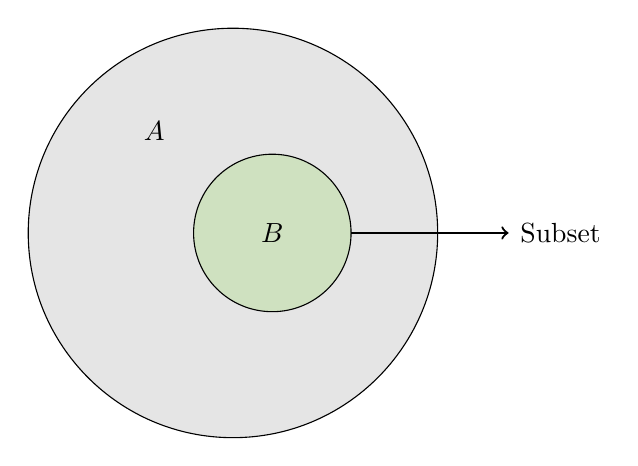
\begin{tikzpicture}
        % Set A
        \draw[fill=gray!20] (0,0) circle (2.6cm);
        \node at (-1,1.3) {$A$};

        % Set B
        \draw[fill=OliveGreen!20] (0.5,0) circle (1cm);
        \node at (0.5,0) {$B$};

        % Subset arrow
        \draw[->, thick] (1.5,0) -- (3.5,0);

        % Subset label
        \node at (4.16,0) {Subset};
    \end{tikzpicture}
    \caption{}
    \label{fig:subset}
\end{figure}

\newpage
\noindent
Written $B \subseteq A$ or $A \supseteq B$, similar to the less than or
equal to signs `$\leq$' and `$\geq$'.

\begin{theo}[Subset]{thm:subset}
    If every element in set $B$ is also in set $A$, then $B$ is a subset of $A$.\\
    Denoted: $B \subseteq A$ or $A \supseteq B$.
\end{theo}

\noindent
\textbf{For Example:}
\begin{itemize}
    \item $\{-1, 0\} \subseteq \{-1, 0, 1, 2, 3\}$
    \item $\{-1, 1, 3\} \subseteq \{-1, 0, 1, 2, 3\}$
    \item $\{-1, 7\} \not\subseteq \{-1, 0, 1, 2, 3\}$
\end{itemize}

\underline{$\not\subseteq$ denotes `not a subset of.'}

\vspace{2em}
\noindent
Explicitly defining a set, say $\{1, 2, 3, ...\}$, is called \textbf{set-roster notation}.\\
\textbf{Set-builder notation} enables us to define the set's properties.

\begin{theo}[Set-Builder Notation]{thm:set_builder}
    Follows the general form: $\{x \mid P(x)\}$,
    \begin{itemize}
        \item $x$ = defines some variable.
        \item $``\mid"$ = is short hand for ``such that.''
        \item $P(x)$ = describes the properties $x$ must satisfy.
    \end{itemize}
\end{theo}

\noindent
\textbf{For Example:} Lets define the set of even integers\\
\begin{itemize}
    \item $\{x \mid x \textnormal{ is an even integer}\}$: ``$x$, such that, $x$ is an even integer.''
    \item $\{x \in \mathbb{Z} \mid x \textnormal{ is even}\}$: ``$x$ in Integers, such that, $x$ is an even.''
    \item $\{x \in \mathbb{Z} \mid x \textnormal{ is not odd}\}$: ``$x$ in Integers, such that, $x$ is not odd.''

\end{itemize}
